\documentclass[10pt]{standalone}
\usepackage{commands}

\begin{document}
    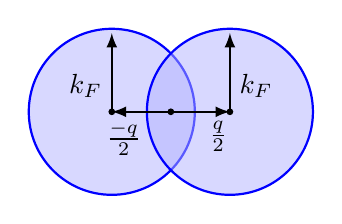
\begin{tikzpicture}
        \draw[blue, thick, fill = white!70!blue, fill opacity=0.5] (-0.75, 0) circle (30pt);
        \draw[blue, thick, fill = white!70!blue, fill opacity=0.5] (0.75, 0) circle (30pt);
        \draw[-latex, thick] (0, 0) -- (0.75, 0);
        \draw[-latex, thick] (0, 0) -- (-0.75, 0);
        \draw[black, fill = black] (0, 0) circle (1pt);
        \draw[black, fill = black] (0.75, 0) circle (1pt);
        \draw[black, fill = black] (-0.75, 0) circle (1pt);
        \node[below] at (0.6, 0) {$\frac{q}{2}$};
        \node[below] at (-0.6, 0) {$\frac{-q}{2}$};
        \draw[-latex, thick] (0.75, 0) -- (0.75, 1);
        \draw[-latex, thick] (-0.75, 0) -- (-0.75, 1);
        \node[right] at (0.75, 0.325) {$k_F$};
        \node[left] at (-0.75, 0.325) {$k_F$};
    \end{tikzpicture}
\end{document}